%!TEX TS-program = xelatex
%!TEX encoding = UTF-8 Unicode

\documentclass[12pt]{extarticle}
% extarticle is like article but can handle 8pt, 9pt, 10pt, 11pt, 12pt, 14pt, 17pt, and 20pt text

\def \ititle {Philosophical Psychology}

\def \isubtitle {Lecture 10}

\def \iauthor {Stephen A. Butterfill}
\def \iemail{s.butterfill@warwick.ac.uk}
\date{}

%for strikethrough
\usepackage[normalem]{ulem}

\input{$HOME/latex_imports/preamble_steve_handout}

%\bibpunct{}{}{,}{s}{}{,}  %use superscript TICS style bib
%remove hanging indent for TICS style bib
%TODO doesnt work
\setlength{\bibhang}{0em}
%\setlength{\bibsep}{0.5em}


%itemize bullet should be dash
\renewcommand{\labelitemi}{$-$}

\begin{document}

\begin{multicols*}{3}

\setlength\footnotesep{1em}


\bibliographystyle{newapa} %apalike

%\maketitle
%\tableofcontents




%---------------
%--- start paste

      
\def \ititle {12: Is There a Role for Motor Processes in Mindreading?}
 
\begin{center}
 
{\Large
 
\textbf{\ititle}
 
}
 
 
 
\iemail %
 
\end{center}
 
 
 
‘There is an early mirror response that is not influenced by the correctness of the movement, 
and a later modulation that differs according to the correctness of the movements reflecting a deeper 
level of [cognitive] processing than the early response’
\citep{naish:2014_effects}.

\begin{center}

  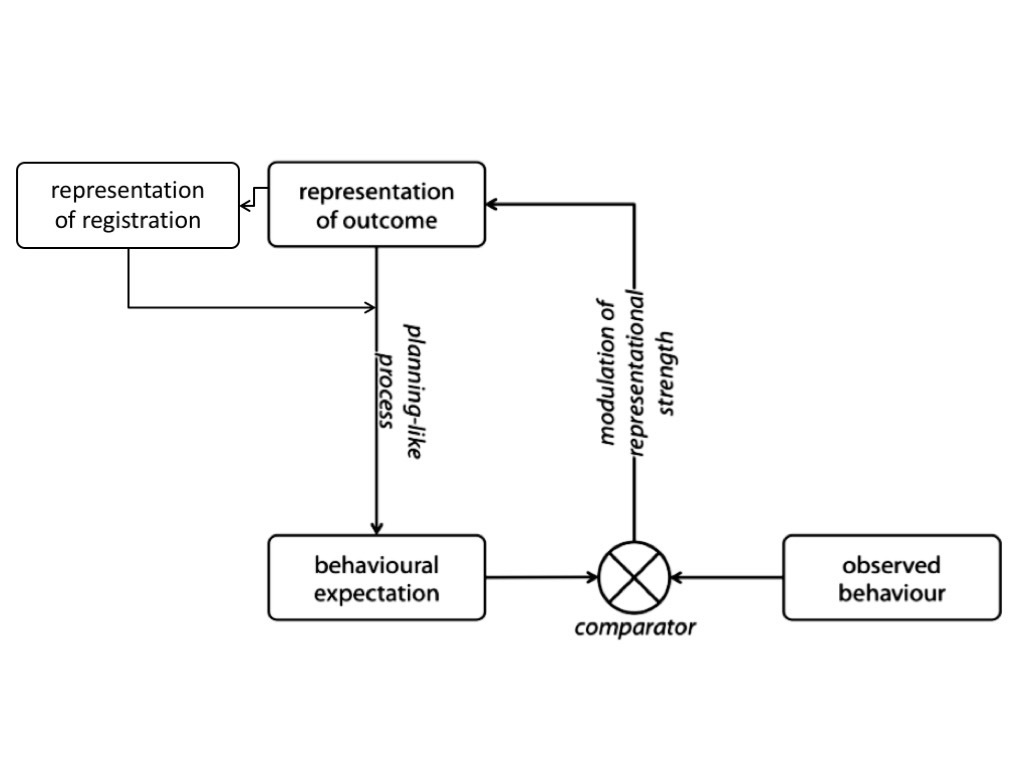
\includegraphics[scale=0.37]{fig/motor_goal_theory.jpg}
  
  \end{center}


Conjecture   1. Automatic belief-tracking depends on outcomes being represented motorically

Conjecture   2. Automatic belief-tracking can influence motor processes that underpin goal-tracking




%--- end paste
%---------------

\footnotesize
\bibliography{$HOME/endnote/phd_biblio}

\end{multicols*}

\end{document}
